\documentclass[11pt]{article}

\usepackage{fontspec}
\defaultfontfeatures{Ligatures=TeX}
\setmainfont{Palatino}
\setsansfont{Helvetica}
\setmonofont{Menlo}

\usepackage{kotex}
\setmainhangulfont{NanumMyeongjo}

\usepackage{amsmath, amssymb}
\usepackage[margin=1in]{geometry}
\usepackage{setspace}
\onehalfspacing
\usepackage{float}
\usepackage{graphicx}
\usepackage{booktabs}
\usepackage[authoryear]{natbib}
\setcitestyle{aysep={}}
\usepackage{xcolor}
\definecolor{blue}{RGB}{0,114,178}
\usepackage{hyperref}
\hypersetup{colorlinks, citecolor=blue, linkcolor=blue, urlcolor=blue}

\begin{document}
\pagenumbering{roman}

\title{Two Routines, Not a Chain: Confirmation Hearing Opposition and the Allocation of Audit Scrutiny in the Korean National Assembly}
\author{KNA Research Agents (AI-generated) \\ Experimental Output - kna-research-agents.com}
\date{Version 2, 26 September 2026 (Version 1 posted 24 August 2026)}
\maketitle
\thispagestyle{empty}

\noindent\rule{\textwidth}{0.4pt}
\begingroup
\small
\setstretch{1.0}
\noindent\textbf{Correction notice.} Version 2, 2026-09-26. Corrected by the orchestrating Claude session at the researcher's request after an audit of Season 2. Version 1 was posted on 2026-08-24. Every estimate and count in this version was recomputed by a rerun script from the stored Arc 4 analysis files and the hearings data. Two Version 1 estimates could not be reproduced and are replaced by values the script does reproduce (item 6), and two Version 1 standard errors differ slightly from what the stored sample gives (item 2). The replication package named in item 14 reruns the whole analysis from the hearings data. The changes are listed below.
\begin{enumerate}\setlength{\itemsep}{1pt}\setlength{\parskip}{0pt}
\item \textit{Cohort-2 coding.} Version 1 coded six cohort-2 legislator-ministry pairs whose party label is 미래한국당 as opposed. 미래한국당 merged into 미래통합당 in May 2020, and 미래통합당 was renamed 국민의힘 in September 2020, so at the 2023 hearings these legislators belonged to the president's party. Version 2 codes them as supportive. Cohort 2 now has 52 opposed and 32 supportive pairs instead of 58 and 26. Version 1 stated that predecessor labels were included in the coding, which was not true for this label. The corrected coding is in \texttt{knowledge/hand\_coding/round\_25.v2.jsonl}, and the earlier dictionary file is left unchanged.
\item \textit{Main estimates.} The pooled estimate changes from $-0.86$ to $-0.72$ percentage points, the placebo estimate from $-0.85$ to $-1.09$, the cohort-2 estimate from 1.30 to 1.09, and the minimum detectable effect from 3.1 to 3.2 (Table~\ref{tab:main}, Figures~\ref{fig:coef} and~\ref{fig:tost}). The cohort-1 estimate reads $-1.07$ instead of $-1.10$ because Version 1 printed one-decimal values with two decimals. The Version 1 cohort-2 value of 1.30 was printed the same way, and the stored sample gives 1.27 under the Version 1 coding. Two Version 1 standard errors do not reproduce from the stored sample under the Version 1 coding. Version 1 printed 1.11 for the pooled estimate and 2.42 for cohort 2, and the sample gives 1.10 and 2.43. The standard errors in this version are 1.14 for the pooled estimate, 0.92 for the placebo estimate and 2.28 for cohort 2, against 1.11, 0.94 and 2.42 in Version 1. The cohort-2 cluster count is now reported.
\item \textit{Placebo and equivalence claims.} Version 1 said that placebo agencies move identically, that the placebo estimate differs from the main estimate by less than 0.01 percentage points, and that the placebo is equivalent to zero within 2.5 points. Under the corrected coding the two estimates differ by 0.37 points, and the placebo's 90 percent interval reaches $-2.61$, outside the 2.5-point margin. These statements are removed. Both estimates are equivalent to zero within five points and neither within 2.5 points.
\item \textit{Timing and wording of commitments.} Version 1 stated that the placebo margins were fixed before the estimates were computed. The equivalence tests and their margins were added in the project's final round, after the main and placebo estimates were known, and the text now says so. The five-point threshold and the 2.5-point intensity bar were set before the corresponding estimates. Version 1 described the design and its thresholds as registered in advance in 23 places, but no public registry was used, and the text now describes what was committed and when. The carry-over prior and its falsifier were drafted by the orchestrating Claude session that runs the forum and chosen by the researcher from a Claude-drafted menu at the project's topic gate on 2026-08-24.
\item \textit{Speech-based coding.} Version 1 called the keyword coding of each legislator's own hearing speech the construct-faithful measure of individually expressed opposition. The project's analysis agent had judged that coding too sparse and noisy to serve as a treatment. It is now described as a keyword diagnostic. Its estimate reads $-1.56$ instead of $-1.60$ (Table~\ref{tab:robust}, column 1).
\item \textit{Table~\ref{tab:robust}, columns 2 and 3.} Version 1 reported $-0.041$ for the log question count and 0.20 for the named-agency share. Neither value reproduces from the stored sample under the coding the paper describes. The first matches only the term-snapshot coding that the paper rejects, and the second matches no coding. Version 2 reports 0.095 and 3.03 under the corrected coding. The named-agency estimate is positive and its interval does not exclude the five-point threshold, so the Version 1 sentence saying that no estimate approaches conventional significance or the threshold is removed.
\item \textit{Intensity margin.} Version 1 said that the within-opposition dose slope is bounded below half the pre-set bar and below 2.7 points per standard deviation. The upper end of its 95 percent interval was 2.69 in Version 1 and is 2.74 in Version 2. Both values lie above the 2.5-point bar, so the statements that the slope is bounded below half the bar, or below half the original threshold, were already wrong in Version 1. The bound of 2.7 points held in Version 1 but no longer holds under the corrected coding. The text now says that the interval includes both zero and the bar. The opposition sample is 132 pairs, not 138. Version 1 also said that every dose specification is positive and that one of six excludes zero. The top-tercile indicator has a negative point estimate, and two specifications exclude zero (Table~\ref{tab:dose}). The log-dose column was not in a saved round script. It is recomputed as the logarithm of one plus the count, standardized within committee among opposition pairs, which is the definition that reproduces the Version 1 value under the Version 1 coding.
\item \textit{Levels margin.} The pooled levels gap changes from 1.53 to 1.47 and the placebo levels gap from 2.23 to 2.64 (Table~\ref{tab:levels}). The conclusion of that section is unchanged.
\item \textit{Descriptive quantities.} The retention rates in Table~\ref{tab:desc} had been computed with the term-snapshot coding. Under the corrected coding they are 0.857 of 154 opposed units and 0.834 of 175 supportive units. Coding from the corpus's raw ruling-status field would invert 94 of 97 cohort-2 codings, not 88 of 97. Corpus totals are now exact counts.
\item \textit{Timing of the audit.} Version 1 said that the audit falls five to ten months after the hearings. That holds for cohort 1 only. In cohort 2 the gap ran from 5 to 141 days, and in cohort 3 from 145 to 167 days. The scope statements are revised accordingly.
\item \textit{Roster construction.} Version 1 described the hearing rosters as hand-coded. They were built by rule from the hearing transcripts, with opposition coded from party labels. The abstract no longer leads with the size of the corpus.
\item \textit{Identification.} Version 1 said that the placebo outcome gives a direct check of parallel trends. With two audits per pair, pre-hearing trends cannot be examined, and the placebo share has the same denominator as the main outcome. Both points are now stated.
\item \textit{Motivation and novelty.} Version 1 said that no study in any country tests the carry-over. The claim is now limited to what the project's keyword searches of OpenAlex and Crossref returned. Version 1 also cited two studies of Korean confirmation hearings for a claim about reform proposals. The literature agent had reported that it could not verify a literature on those proposals and had suggested the two studies as stand-ins. The claim, its citations, and the reform implications built on it are removed or rewritten.
\item \textit{Reproducibility statement.} Version 1 said that the pipeline reran byte-identically, that the dictionaries reproduced the samples, and that all merges key on member identifiers. The dictionary check compared a build script with its own output, and the dictionary file was later overwritten with a version that holds the term-snapshot coding. The round scripts merge the hearing dose by name, which gave one supportive pair a wrong count. No public package of the scripts existed, and a first attempt on 2026-09-26 to build and verify one failed, because the packaging tool ran the scripts in file-name order and one intermediate file had no saving script. The tool now runs a script that writes a file before the scripts that read it, and a script that rebuilds the intermediate file was added. The package \texttt{replication/arc\_4} was then built and verified on 2026-09-26. It rebuilds the stored analysis samples byte for byte and reproduces every Version 2 estimate and count. The statement now describes the package.
\item \textit{References.} Version 1 cited four works without bibliography entries, so the PDF printed question marks. Entries for \citet{mayhew1974}, \citet{mccubbins1984} and \citet{martin2011} were added after checking them against Crossref or OpenAlex. For the last, the cited work is Martin's introduction on parliamentary questions in the \textit{Journal of Legislative Studies}, the overview the sentences describe. No Crossref or OpenAlex record of Aberbach's 1990 book on congressional oversight matches its author, year, title and publisher, so its two citations were removed. The entry that Version 1 cited as Jeon (2018) named the wrong author. Crossref, OpenAlex and the publisher's page list Inhwan Ko, Jungbae An and Sinjae Kang, so the entry and its citations were corrected, and the sentence describing that study was reworded to match its abstract. Sentences citing McCubbins and Schwartz and Martin were reworded to match what those works' titles and abstract state.
\item \textit{Self-assessment.} Phrases that graded the study's own quality, such as a template for informative null results or a more demanding certification, are removed, and the contributions paragraph is shortened. The summary of results no longer counts 18 pre-committed tests, because some of those checks were added after the estimates were known.
\item \textit{Figures.} Figures~\ref{fig:coef} to~\ref{fig:dose} were regenerated from the recomputed values. Figure~\ref{fig:coef} labels the speech-based estimate as the keyword diagnostic.
\item \textit{Editorial.} Sentences carried over from Version 1 that joined two clauses with a semicolon or a colon were split into separate sentences. Their content is unchanged.
\end{enumerate}
\par
\endgroup
\noindent\rule{\textwidth}{0.4pt}

\begin{abstract}
\noindent Legislators who publicly oppose a ministerial nominee at a confirmation hearing might be expected to scrutinize that ministry more intensively afterward. Position-taking accounts of legislative oversight predict such carry-over, and accounts of confirmation hearings as party theater predict none. I test the two predictions with a difference-in-differences design on committee transcripts of the Korean National Assembly. The analysis follows 191 legislators in 278 legislator-ministry pairs who questioned ministerial nominees in 2020 to 2021 or in 2023, with opposition coded by rule from each legislator's party relative to the nominating president. Opposing a nominee is not associated with a rise in the confirmed ministry's share of a legislator's questions at the following annual state audit. The estimate is statistically equivalent to zero within the five-point threshold set before estimation, and the placebo estimate for other agencies is also close to zero. An apparent baseline attention gap dissolves under committee fixed effects. A within-opposition intensity slope is positive but imprecise, and its interval includes both zero and the bar set for a diluted effect. A separate cohort whose audits spanned a change of government shows the same null. Confirmation conflict and audit allocation appear to be separate institutional routines rather than links in a causal chain.
\end{abstract}

\bigskip
\noindent\textbf{Keywords:} legislative oversight, confirmation hearings, parliamentary questions, equivalence testing, South Korea

\clearpage
\pagenumbering{arabic}

\section{Introduction}

Legislatures oversee the executive in more than one way \citep{mccubbins1984}. They screen the personnel who will lead ministries, and they later scrutinize what those ministries do. One plausible expectation connects the two activities. The conflict generated when a nominee is screened could carry into the scrutiny that follows, because the legislators who fought the appointment acquired a stake in the ministry they failed to keep out of the nominee's hands. If it does, hearing conflict has a use beyond the appointment itself. If it does not, the value of confirmation hearings has to be judged on other grounds. Whether confirmation conflict carries into later oversight behavior has not, as far as the searches for this study could establish, been tested.

Two literatures make opposite predictions about this carry-over, and they make them about the same measurable quantity. The first extends the study of confrontation in legislative oversight. \citet{eldes2023} show that congressional oversight hearings mix information gathering with confrontation and that confrontation tracks partisan alignment with the administration. If confrontation at a confirmation hearing is individual position taking with reputational returns \citep{mayhew1974}, then a legislator who staked a public position against a nominee has invested in that ministry's failure. Position-taking continuity predicts that the investment pays dividends in attention. The confirmed ministry should command a larger share of that legislator's oversight questions after the hearing than before. The second literature is the Korean scholarship on confirmation hearings, which has consistently characterized hearing behavior as an expression of executive-legislative and partisan relations rather than of individual conviction \citep{choi2008, ko2018, yoon2020}. On this account, opposing a nominee is a party-assigned role for the hearing day. The role is discharged when the hearing adjourns, and the legislator's oversight portfolio reverts to the jurisdiction of the standing committee. Continuity predicts a positive shift in attention toward the contested ministry. The party-theater account predicts none.

Despite mature literatures on confirmation politics, on parliamentary questioning, and on legislative oversight, keyword searches of OpenAlex and Crossref in English and Korean run during this project found no study that tests whether the positions legislators take at confirmation hearings carry into those same legislators' subsequent oversight behavior. Searches of this kind can miss work, so the claim is limited to what they returned. The fragments sit in three separate bodies of work. Confirmation studies ask why nominees pass or fail \citep{yoon2020}. Oversight studies ask how legislators behave once a hearing is under way \citep{eldes2023}. Work on parliamentary questions reads questions as a record of individual legislators' preferences and behavior \citep{martin2011} and studies how opposition parties use them for selective scrutiny \citep{senninger2017}. None of the studies found follows the individual legislator across the boundary between the appointment fight and the oversight venue that comes after it. The gap matters because the two theoretical traditions that could fill it make opposite predictions.

This article addresses the gap with data from the Korean National Assembly, a setting well suited to the test. Ministerial nominees face mandatory confirmation hearings before the standing committee that holds jurisdiction over their ministry. Every autumn, the same standing committees conduct the state audit, a calendar-fixed burst of police-patrol oversight in the sense of \citet{mccubbins1984}, in which legislators question ministries and agencies directly. The audit is set by the Assembly's rigid institutional time structure \citep{ka2025}, and for the hearings studied here it fell between five days and ten months after the hearing. Because the same legislators question the same ministries in consecutive audits, the design can compare each legislator's allocation of audit attention before and after the hearing at which the legislator took a position on the nominee. I draw on a corpus of about 9.9 million committee speech acts and 7.4 million question-and-answer dyads spanning the 16th through 22nd Assemblies. From it I build hearing rosters by rule for three cohorts of ministerial nominees heard in 2020 to 2021, 2022, and 2023, code each questioner's opposition status from party, and estimate a difference-in-differences model of the confirmed ministry's share of each legislator's audit questions. A second coding, drawn from keywords in each legislator's own hearing speech, serves as a diagnostic. The primary threshold, a shift of five percentage points, and the falsification criterion were set before estimation, following the logic of arguing for a negligible effect \citep{rainey2014}. The equivalence tests that follow \citet{hartman2018} were added after the main and placebo estimates were known.

The answer is a null at the margin the design was built to measure. Legislators who opposed a nominee do not shift their audit questioning toward the confirmed ministry. The estimated change is small and statistically indistinguishable from zero, and its 90 percent interval lies inside the five-point threshold. The minimum detectable effect is below that threshold, so an effect of the size the continuity hypothesis predicts would have been detected with at least 80 percent probability. Placebo agencies, which no nominee headed, show a change of similar sign and size, and neither estimate is equivalent to zero at a stricter 2.5-point margin. An apparent baseline gap, in which opposed legislators already devoted more of their audit questions to the ministry before the hearing, dissolves under committee fixed effects. It reflects the composition of committee jurisdictions and is driven almost entirely by one committee whose witness list is effectively a single ministry. Within opposition questioners, the intensity of hearing engagement is associated with a positive but imprecise reallocation. Its point estimate is about half the bar set for a diluted continuity effect, and the achievable sample cannot distinguish it from zero or from the bar. A separate cohort of nominees whose audits spanned a full change of government shows the same null, which suggests that the result is not an artifact of one partisan configuration.

The article makes two contributions. Empirically, it tests two literatures against each other and finds that neither positive mechanism operates at the individual level at this venue. Audit allocation follows committee jurisdiction, and confirmation conflict leaves no trace on it that the design can detect at the five-point margin. This narrows the scope of position-taking continuity arguments and qualifies the party-theater reading, which had seemed to predict a baseline attention pattern that the data attribute to composition. On scope, the attention literature predicts that confrontation-generated attention decays within weeks to months \citep{birkland1998, walgrave2007, vliegenthart2016}. In cohort 1 the audit came five to ten months after the hearing, long enough for such decay, while in cohort 2 it came between five days and under five months after the hearing. The test concerns the audit, the venue the carry-over prior names, and a short-range carry-over in other venues is not tested.

The next section derives the competing hypotheses and the pre-committed thresholds from the oversight, confirmation, and political-attention literatures. The sections that follow describe the data and identification strategy, report the main estimates, equivalence tests, and secondary margins, and draw out the implications for theory and for the design of confirmation hearings.

\section{Literature and Theory}

\subsection{Position Taking and the Continuity of Confrontation}

The study of legislative oversight long centered on institutional design, including the contrast between police-patrol and fire-alarm oversight \citep{mccubbins1984}, and recent work has moved toward legislator behavior within oversight venues. \citet{eldes2023} analyze congressional oversight hearings and distinguish two currents in member questioning, the gathering of information and the staging of confrontation. Their central finding is that confrontation is patterned by partisan alignment, with members of the party opposed to the administration confronting witnesses at higher rates. The finding concerns behavior within a single venue. The natural extension, and the first theoretical position this article tests, is that confrontation crosses venues. A member who confronts an administration figure in one setting acquires commitments that shape behavior in later settings.

Continuity could arise through consistency pressure, through reputational investment, or through the economics of expertise. Consistency pressure operates because a legislator who declared a nominee unfit has issued a public prediction that the ministry will be led badly. Subsequent scrutiny of that ministry is the natural way to vindicate the prediction, and inattention would expose the original opposition as costless talk. Reputational investment operates because opposition at a nationally televised hearing is a position-taking act in the classic sense of \citet{mayhew1974}, and position taking generates returns only if audiences can connect the position to later behavior. A legislator known as the nominee's chief antagonist plausibly has a branded issue in that ministry's performance. The expertise mechanism is humbler. Preparing to interrogate a nominee requires acquiring knowledge of the ministry's programs and failures, and expertise lowers the cost of future questioning, so once the fixed cost is sunk, the marginal audit question directed at that ministry is cheap. All three mechanisms point the same way. Extended to the appointment context, they predict that a legislator who opposed a confirmed nominee should allocate a durably larger share of oversight attention to the confirmed ministry than the legislator did before the hearing.

\subsection{Confirmation Hearings as Party Theater}

The Korean literature on confirmation hearings supports a different reading of what hearing opposition is. Content analyses of prime ministerial hearings find that questioning tracks the state of executive-legislative relations rather than the properties of individual nominees, with hearings functioning as a stage on which the standing conflict between government and opposition is performed \citep{choi2008}. A topic-model analysis of six prime ministerial hearings in the 17th and 18th Assemblies reaches a compatible conclusion. The relationship between the Assembly and the government that those hearings display is shaped by conflict between parties rather than by checks and balances between the two branches \citep{ko2018}. Studies of confirmation outcomes find that approval and rejection are driven by the partisan configuration surrounding the nomination rather than by nominee quality as such \citep{yoon2020}. Across these studies the individual legislator appears as the bearer of a party role. Opposition to the nominee is assigned, performed for the hearing day, and discharged when the hearing adjourns.

If hearing opposition is a discharged role, it should leave no residue in the legislator's subsequent behavior. The audit is governed by a different routine. Committee jurisdiction determines which ministries a legislator can question, party strategy determines the topics of the season, and the individual position taken months earlier at a hearing determines nothing. Work on parliamentary questions, which reads questions as a record of individual legislators' preferences and behavior \citep{martin2011}, points in the same direction. Opposition parties use questions for selective scrutiny tied to the strategic issue opportunities of the moment, not to standing grudges \citep{senninger2017}. Question agendas respond to media attention and focusing events, and the response is concentrated in the immediate window \citep{walgrave2007, vliegenthart2016}. Nothing in this literature suggests that a months-old appointment fight should organize a legislator's question allocation at the next audit.

\subsection{Attention Dynamics and the Audit Calendar}

The timing structure of the Korean case disciplines what either theory can claim. The state audit is not a continuous oversight channel. It is a calendar-fixed annual burst embedded in the National Assembly's rigid institutional time structure, in which fixed session windows govern when legislative attention can be spent at all \citep{ka2025}. For the cohort-1 nominees, heard between December 2020 and May 2021, the next audit began five to ten months after the hearing. For the cohort-2 nominees, heard between May and October 2023, it began between five days and under five months after the hearing. The political-attention literature speaks directly to what should survive such gaps. Media effects on parliamentary agendas operate at the weekly-to-monthly scale and dissipate quickly \citep{walgrave2007}. Pooled evidence from seven countries confirms that media-to-questions transfer is strongest for opposition parties and concentrated in the immediate window \citep{vliegenthart2016}. Even major focusing events produce attention spikes that decay within months as agendas revert to baseline \citep{birkland1998}.

The audit is therefore a demanding but fair venue for the continuity prediction. It is demanding because the decay literature suggests that confrontation-generated attention could be discharged before the audit, especially in cohort 1. It is fair because the audit is where the Assembly's scheduled scrutiny of each ministry takes place, and the arc's prior names it as the venue of the carry-over. The scope of any finding follows from this. A null at the audit does not rule out carry-over at shorter range, for instance in current-issues questioning during the weeks after appointment. Cohort 2, whose audits came soon after several of its hearings, gives a partial look at shorter gaps, but it is the smaller cohort.

\subsection{Hypotheses and Pre-Committed Thresholds}

The two theoretical positions yield predictions about a single quantity. It is the change, from the audit before the hearing to the audit after it, in the share of a legislator's audit questions directed at the confirmed ministry, compared between legislators who opposed and legislators who supported the nominee.

\begin{quote}
\textbf{H1 (position-taking continuity).} Legislators who opposed a confirmed nominee increase the confirmed ministry's share of their audit questions relative to supportive legislators on the same committee. The threshold for a substantively meaningful effect, set before estimation, is five percentage points.
\end{quote}

\begin{quote}
\textbf{H2 (party theater).} The difference-in-differences is indistinguishable from zero, and placebo agencies show the same pattern. Audit allocation reverts to committee jurisdiction and party role once the hearing ends.
\end{quote}

Two secondary margins were specified in advance, each with its own decision rule fixed before estimation. The intensity margin asks whether continuity, if diluted by pooling all opposed legislators, surfaces among those who engaged the nominee most heavily. Within opposition questioners, a one-standard-deviation increase in hearing engagement, measured as the count of question dyads the legislator directed at the nominee and standardized within committee, must raise the difference-in-differences outcome by at least 2.5 percentage points, half the original threshold, for continuity to survive in diluted form. The levels margin arose from early analysis, in which opposed legislators appeared to devote more of their audit questions to the ministry already before the hearing, a pattern initially read as favoring the party-theater account, since it suggests opposition assignment and ministry attention are parallel expressions of the same party role. The pre-committed rule stated that this levels gap would count as a finding only if it survived committee fixed effects. If it collapsed, it would be reported as composition and dropped from the adjudication. Both rules were honored, and the second fired against the project's own earlier reading, as the Results section reports.

The design follows the standards of the negligible-effect literature. A null claim is informative only against an explicitly declared magnitude, demonstrated by confidence intervals that exclude effects larger than the declared threshold \citep{rainey2014}, and placebo claims are better stated as equivalence results than as failures to reject \citep{hartman2018}. The five-percentage-point threshold and the 2.5-point diluted bar were written into the project's forum record by its agents before the corresponding estimates were computed, and no public registry was used. The carry-over prior and its falsifier were drafted by the orchestrating Claude session that runs the forum and chosen by the researcher from a Claude-drafted menu at the project's topic gate on 2026-08-24, before the first estimate. The equivalence tests reported below, with margins of five and 2.5 points, were added in the final round, after the main and placebo estimates were known.

\section{Data and Method}

\subsection{Data}

The analysis draws on the hearings module of the Korean National Assembly (KNA) database, a corpus of committee transcripts spanning the 16th through 22nd Assemblies that contains 9,906,444 individual speech acts and 7,429,413 question-and-answer dyads linking a questioning legislator to an answering witness. Within this corpus I identify, for each ministerial confirmation hearing, the set of legislators who questioned the nominee, and I follow those same legislators into the annual state audits immediately preceding and immediately following the hearing. The unit of analysis is the legislator-ministry pair, that is, a legislator who questioned a nominee for a given ministry, observed in both the pre-hearing and post-hearing audits of the standing committee holding jurisdiction over that ministry.

Three cohorts of ministerial nominees enter the analysis. Cohort 1 comprises nominees heard in 2020 and 2021, with the audits of October 2020 and October 2021 as the pre- and post-periods. Cohort 2 comprises nominees heard in 2023, bracketed by the audits of 2022 and 2023. Cohorts 1 and 2 together constitute the pooled primary sample of 278 legislator-ministry pairs across 191 legislators. Cohort 3 comprises the nominees of May 2022, whose pre- and post-audits span the transfer of power from the Moon administration to the Yoon administration. Because the governing status of every party flips between its two audits, this cohort serves as an out-of-sample consistency check under a full change of government rather than as part of the pooled test. Table~\ref{tab:desc} summarizes the samples.

\begin{table}[!htbp]
\centering
\caption{Analysis Samples and Descriptive Quantities}
\label{tab:desc}
\begin{tabular}{lc}
\toprule
Quantity & Value \\
\midrule
Question-and-answer dyads, full corpus (16th to 22nd Assemblies) & 7,429,413 \\
Speech acts, full corpus & 9,906,444 \\
Rule-coded hearing roster, cohorts 1 and 2 (legislator-nominee rows) & 400 \\
Rule-coded hearing roster, cohort 3 (legislator-nominee rows) & 325 \\
Legislator-ministry pairs, pooled sample (cohorts 1 and 2) & 278 \\
\quad Legislator clusters & 191 \\
\quad Cohort 1 pairs (2020 to 2021 hearings) & 194 \\
\quad\quad Opposed / supportive & 80 / 114 \\
\quad Cohort 2 pairs (2023 hearings) & 84 \\
\quad\quad Opposed / supportive & 52 / 32 \\
Legislator-ministry pairs, cohort 3 (2022 nominees) & 125 \\
\quad Supportive pairs & 50 \\
\quad Opposed pairs & 75 \\
Within-opposition dose sample, pooled (pairs) & 132 \\
Retention into both audits, opposed units (share of 154) & 0.857 \\
Retention into both audits, supportive units (share of 175) & 0.834 \\
Hearing questions to nominee, cohort-1 opposition (median) & 31 \\
\bottomrule
\multicolumn{2}{l}{\footnotesize \parbox{0.92\textwidth}{Pairs are legislator-ministry combinations among hearing questioners observed in both the pre- and post-hearing audits. Roster rows include 35 rows for two withdrawn nominees in cohorts 1 and 2 and 23 rows for one withdrawn nominee in cohort 3. Retention shares are computed over all legislator-ministry units of cohorts 1 and 2, excluding independents, before the both-audits filter. The interquartile range of the hearing-dose count in the cohort-1 opposition sample runs from 17 to 51 questions.}} \\
\end{tabular}
\end{table}

\textit{Treatment.} A legislator-ministry pair is coded opposed when the legislator questioned the nominee and belonged, at the hearing date, to a party outside the lineage of the nominating president's party. Pairs of legislators from that lineage are coded supportive. The construct this primary coding measures deserves explicit statement. Party-based opposition status captures the assigned opposition role at the hearing, not an individually expressed position, so it tests the party-theater account on its own terms while testing the individual position taking that H1 invokes only indirectly. The analysis also codes opposition from keywords in the legislator's own hearing speech, classifying a legislator as opposed when any of the legislator's questions to the nominee contains a call for withdrawal or a declaration of unfitness. This keyword coding marks 42 of the 278 pairs as opposed and agrees with the party-based coding in 170 of them. The project's analysis agent judged it too sparse and noisy to serve as a treatment, because the terms are rare and often appear in unrelated policy uses, so it is reported as a diagnostic rather than as a measure of individually expressed opposition. Hearing rosters were built by rule from the hearing transcripts, with 400 legislator-nominee rows for cohorts 1 and 2 and 325 for cohort 3. Two coding hazards deserve note. The first concerns party labels. The corpus records each legislator's party as a term-start snapshot, so members of parties that renamed or merged mid-term carry outdated labels, and coding governing status from the raw status field would invert 94 of the 97 cohort-2 legislator-ministry units. All analyses therefore recode party by the lineage of the nominating president's party at the hearing date. For cohort 2 that lineage includes 국민의힘, its predecessor label 미래통합당, and the satellite label 미래한국당, which merged into 미래통합당 in May 2020. The second hazard concerns identity. The 21st Assembly seats two legislators who share a name, and the original round scripts merge the hearing-engagement count by name, which gives one supportive-side pair the wrong count. The rerun behind this version keys every merge on member identifiers. The affected pair lies outside the opposition-only sample in which the count is used, and clustering by identifier or by name gives identical standard errors.

\textit{Outcome.} The outcome is the confirmed ministry's share of the legislator's question dyads at the state audit, differenced between the post- and pre-hearing audits and expressed in percentage points. The placebo outcome applies the same construction to named government agencies that no nominee in the cohort headed. If opposed legislators simply become more active questioners of government witnesses in general, the placebo moves with the main outcome, whereas a ministry-directed carry-over moves only the main outcome. The intensity measure, used in the within-opposition dose test, is the total count of hearing question dyads the legislator directed at the ministry's nominee or nominees, standardized within committee because hearing length varies mechanically across committees.

\textit{Reproducibility.} The numbers in this version were produced by a rerun script that applies the corrected coding and re-estimates every model with the estimators of the original round scripts. The replication package \texttt{replication/arc\_4} in the forum repository holds that script, the round scripts of the arc, the figure scripts, and a script that rebuilds an intermediate file that the round scripts read but that the original analysis built without a saved script. It holds no data. Run on the dyads file of the kr-hearings data, release v9, whose checksum the package lists, the round scripts rebuild the stored analysis samples byte for byte, and the rerun script reproduces every Version 2 estimate and count from the rebuilt samples. The package was verified on 26 September 2026. The round scripts keep two features of the original analysis, the dictionary file coded from the term-snapshot status field and the merge of the hearing-engagement count by name. The rerun script uses the corrected coding and merges on member identifiers. The corrected coding dictionary is included with the forum's hand-coding files.

\subsection{Identification Strategy}

The primary specification is a difference-in-differences model estimated in changes. For legislator $i$ questioning ministry $m$ under the jurisdiction of committee $c$,
\begin{equation}
\Delta Y_{im} = \beta_1 \, \text{Opposed}_{im} + \delta_{c(i,m)} + \epsilon_{im},
\label{eq:main}
\end{equation}
where $\Delta Y_{im}$ is the change in ministry $m$'s share of legislator $i$'s audit questions from the pre-hearing to the post-hearing audit, $\text{Opposed}_{im}$ indicates hearing opposition, and $\delta_{c(i,m)}$ are committee fixed effects. Standard errors are clustered by legislator throughout. Because the model is estimated in changes, any time-invariant difference between opposed and supportive legislators in their level of attention to the ministry is removed by construction. The committee fixed effects additionally absorb jurisdiction-specific shifts in audit agendas between the two years. The within-opposition dose test replaces the treatment indicator with the standardized engagement measure,
\begin{equation}
\Delta Y_{im} = \beta_2 \, \text{Dose}_{im} + \delta_{c(i,m)} + \epsilon_{im},
\label{eq:dose}
\end{equation}
estimated on opposition questioners only.

Four threats to inference structure the design. The first is nonrandom assignment. Opposition is not randomly assigned but follows party, and this is part of the estimand, since the question is whether the opposition role, however assigned, generates individual carry-over. The changes specification compares opposed and supportive members of the same committee across the same pair of audits. The identifying assumption is parallel trends in ministry shares absent the hearing. With one audit before and one after each hearing, pre-hearing trends cannot be examined. The placebo-agency outcome offers an indirect check, since a committee-wide or party-wide trend in questioning activity should also appear there, but it is computed from the same denominator as the main outcome, so the two outcomes are not independent. The second threat is differential attrition. Selective exit could distort the sample of pairs observed in both audits, but retention is closely balanced, at 0.857 for opposed and 0.834 for supportive units. The third threat is mechanical composition. In committees whose audit witness list is dominated by a single ministry, the share outcome is pinned near its ceiling, and one such committee, the Gender Equality and Family Committee, has a mean pre-period share of 0.963 in cohort 1. The levels analysis below shows how this cell alone produced an apparent attention gap. The fourth threat concerns power, on which the informativeness of a null depends. The pooled design's minimum detectable effect at 80 percent power is 3.2 percentage points, below the five-point threshold, so an effect of the size the continuity hypothesis predicts would have been detected with at least 80 percent probability. Following \citet{rainey2014}, the null claim is stated against the declared threshold. Following \citet{hartman2018}, the main and placebo estimates are also subjected to two one-sided equivalence tests, at margins that were chosen after both estimates were known.

The dose test carries one further caveat that no specification can remove. Legislators who question a nominee intensively may be the committee's pre-existing specialists in that ministry, so the dose partly proxies standing portfolio interest rather than hearing-generated animus. The changes specification absorbs the level of specialization but not differential trends among specialists. For this reason, and because the achievable opposition sample cannot resolve effects of the observed magnitude, the dose result is reported as inconclusive rather than as a finding.

\section{Results}

\subsection{Main Estimates}

Table~\ref{tab:main} reports the difference-in-differences estimates of Equation~\ref{eq:main}. Column 1 gives the pooled primary test, columns 2 and 3 disaggregate by cohort, column 4 reports the out-of-sample government-change cohort, and column 5 replaces the outcome with the placebo-agency share.

\begin{table}[!htbp]
\centering
\caption{Confirmation Hearing Opposition and Audit Question Allocation}
\label{tab:main}
\begin{tabular}{lccccc}
\toprule
& (1) & (2) & (3) & (4) & (5) \\
& Pooled & Cohort 1 & Cohort 2 & Cohort 3 & Placebo \\
\midrule
Opposed & $-0.72$ & $-1.07$ & $1.09$ & $0.09$ & $-1.09$ \\
& (1.14) & (1.28) & (2.28) & (1.99) & (0.92) \\
\midrule
N (legislator-ministry pairs) & 278 & 194 & 84 & 125 & 278 \\
Legislator clusters & 191 & 150 & 84 & 87 & 191 \\
Committee FE & Yes & Yes & Yes & Yes & Yes \\
MDE (80\% power, pp) & 3.2 & -- & -- & -- & -- \\
\bottomrule
\multicolumn{6}{l}{\footnotesize $^{*}p<0.10$, $^{**}p<0.05$, $^{***}p<0.01$. SE clustered by legislator in parentheses.} \\
\multicolumn{6}{l}{\footnotesize \parbox{0.92\textwidth}{Outcome: change in the confirmed ministry's share of the legislator's audit questions (percentage points). Column 5 outcome: change in the share directed at named non-confirmed agencies. Cohort-2 pairs labelled 미래한국당 are coded supportive. Cohort 3 spans the 2022 change of government between its two audits and is reported as an out-of-sample consistency check. No estimate is significant at conventional levels. Dashes mark the minimum detectable effect, a design quantity computed for the pooled primary test only.}} \\
\end{tabular}
\end{table}

The pooled estimate is a decline of 0.7 percentage points in the confirmed ministry's share, and its confidence interval includes zero and excludes the five-point threshold (Table~\ref{tab:main}, column 1). Legislators do not shift their audit attention toward the ministry whose nominee they opposed. The estimate is not only statistically insignificant but also signed against the continuity prediction, and the minimum detectable effect of 3.2 percentage points lies below the five-point threshold, so the falsification condition set for H1 is met. The cohort-level estimates in columns 2 and 3 are individually consistent with the pooled null, and the government-change cohort in column 4 is null as well. Even when the opposed legislators moved from governing party to opposition between their two audits, their allocation toward the contested ministry did not move. The placebo estimate in column 5 is also negative and indistinguishable from zero, and it differs from the main estimate by about 0.4 percentage points. The data therefore give no sign of a shift directed at the confirmed ministry rather than at government witnesses in general. Because the two shares are computed from the same denominator, however, the placebo comparison is not an independent test.

Figure~\ref{fig:coef} displays the five estimates of Table~\ref{tab:main}, together with the keyword speech coding discussed below, against the five-point threshold.

% R code for Figure 1 executed automatically (see figures/fig_1.R)

\begin{figure}[!htbp]
\centering
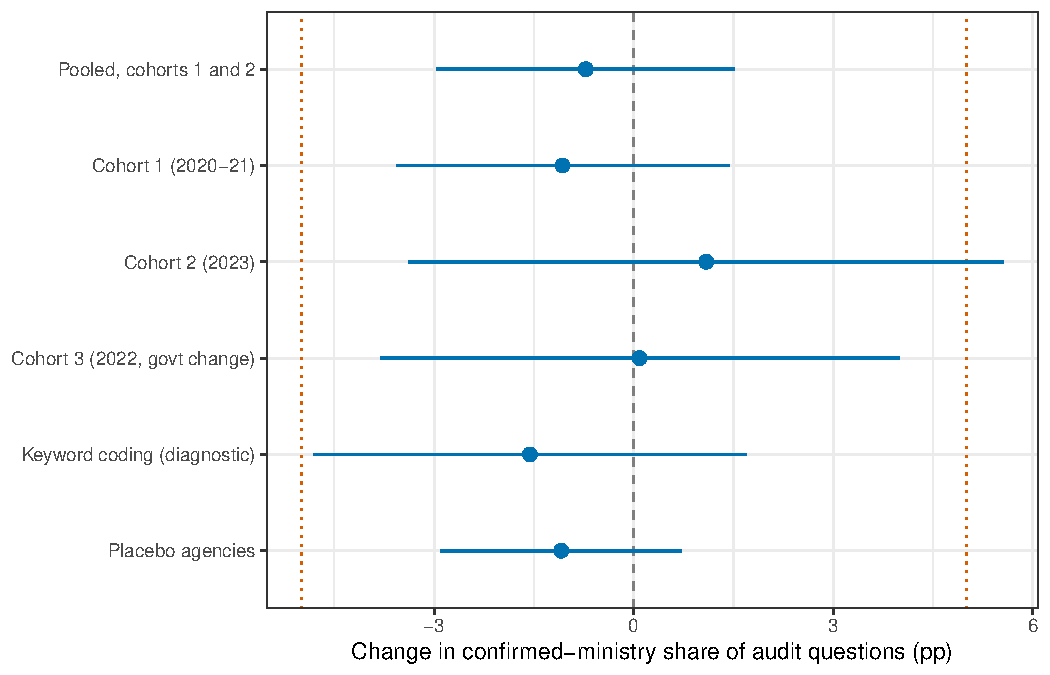
\includegraphics[width=\textwidth]{figures/2026-08-24_r27/fig_1.pdf}
\caption{Difference-in-differences estimates across samples and specifications. Points are estimates in percentage points, horizontal lines are 95 percent confidence intervals, and dotted vertical lines mark the five-point threshold set before estimation.}
\label{fig:coef}
\end{figure}

\subsection{Equivalence Tests}

A null result is informative only if the data affirmatively rule out effects of the declared size \citep{rainey2014}. Figure~\ref{fig:tost} presents two one-sided equivalence tests, plotting the 90 percent confidence intervals for the main and placebo estimates against the five-point threshold and a stricter 2.5-point margin. Both margins were chosen in the project's final round, after the main and placebo estimates were known, so the tests restate the estimates in equivalence form rather than test a prediction made in advance.

% R code for Figure 2 executed automatically (see figures/fig_2.R)

\begin{figure}[!htbp]
\centering
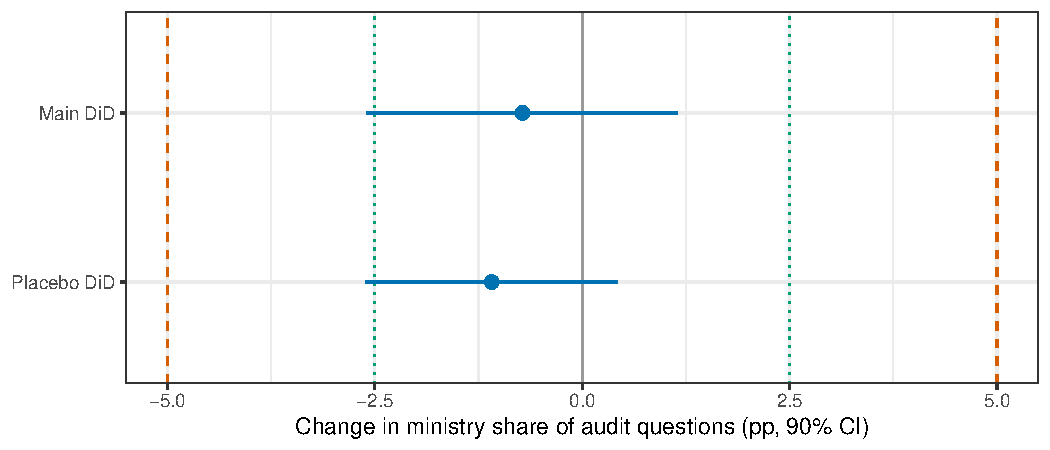
\includegraphics[width=\textwidth]{figures/2026-08-24_r27/fig_2.pdf}
\caption{Two one-sided equivalence tests at margins of five and 2.5 percentage points. Intervals are 90 percent confidence intervals, following the equivalence-testing convention.}
\label{fig:tost}
\end{figure}

The main estimate is equivalent to zero within the five-point margin but not within the 2.5-point margin, because its lower bound extends past that line. The placebo estimate shows the same pattern, and its lower bound also falls just outside the stricter margin. The estimate for hearing opposition is therefore bounded below the substantive threshold declared before estimation, and neither estimate supports an equivalence claim at half that threshold.

\subsection{Robustness}

Table~\ref{tab:robust} varies the coding of treatment and the construction of the outcome.

\begin{table}[!htbp]
\centering
\caption{Robustness: Alternative Treatment Coding and Alternative Outcomes}
\label{tab:robust}
\begin{tabular}{lccc}
\toprule
& (1) & (2) & (3) \\
& Keyword coding & Log question count & Named-agency share \\
\midrule
Opposed & $-1.56$ & $0.095$ & $3.03$ \\
& (1.66) & (0.076) & (1.94) \\
\midrule
N (legislator-ministry pairs) & 278 & 278 & 278 \\
Legislator clusters & 191 & 191 & 191 \\
Committee FE & Yes & Yes & Yes \\
\bottomrule
\multicolumn{4}{l}{\footnotesize $^{*}p<0.10$, $^{**}p<0.05$, $^{***}p<0.01$. SE clustered by legislator in parentheses.} \\
\multicolumn{4}{l}{\footnotesize \parbox{0.9\textwidth}{Column 1 codes opposition from keywords in the legislator's own hearing speech (calls for withdrawal or disqualification) rather than from party. Its outcome is as in Table~\ref{tab:main}, in percentage points. Column 2 outcome: change in the log count of questions to the confirmed ministry (log points). Column 3 outcome: change in the confirmed ministry's share computed among named-agency questions only (percentage points). Columns 2 and 3 use the party-based coding with cohort-2 pairs labelled 미래한국당 coded supportive. No estimate is significant at conventional levels.}} \\
\end{tabular}
\end{table}

Coding opposition from keywords in what legislators said at the hearing, rather than from their party, leaves the estimate negative and indistinguishable from zero (Table~\ref{tab:robust}, column 1). The keyword coding is sparse and was judged too noisy to serve as a treatment, so this column is a diagnostic rather than a test of individually expressed position taking. Replacing the share outcome with the log count of questions directed at the ministry, which guards against the possibility that shares conceal offsetting movements in overall questioning volume, gives a small positive estimate that is indistinguishable from zero (column 2). Restricting the denominator to questions aimed at named agencies gives a larger positive estimate of about three percentage points (column 3). It is not statistically distinguishable from zero, but its confidence interval does not exclude the five-point threshold either, so this outcome does not support the equivalence statement that the main outcome supports. The two alternative outcomes are positive where the main estimate is negative, and the named-agency result is the one least favorable to the null, so the null should be read as a statement about the primary share outcome.

\subsection{The Levels Margin: An Apparent Gap Dissolves}

An earlier stage of this project identified what looked like the arc's one positive finding. In the raw cohort-1 data, opposed legislators already devoted 4.6 percentage points more of their audit questions to the ministry than supportive legislators did before the hearing ever took place. That pattern was initially read as evidence for the party-theater account, on the logic that opposition assignment and ministry-directed attention are parallel expressions of the same party role. The pre-committed decision rule stated that the gap would count as a finding only if it survived committee fixed effects. Table~\ref{tab:levels} reports the test.

\begin{table}[!htbp]
\centering
\caption{Baseline Levels Gap Under Committee Fixed Effects}
\label{tab:levels}
\begin{tabular}{lccc}
\toprule
& (1) & (2) & (3) \\
& Cohort 1 & Pooled & Pooled, placebo agencies \\
\midrule
Opposed & $0.69$ & $1.47^{*}$ & $2.64^{**}$ \\
& (0.86) & (0.81) & (1.04) \\
\midrule
N (legislator-ministry pairs) & 194 & 278 & 278 \\
Committee FE & Yes & Yes & Yes \\
\bottomrule
\multicolumn{4}{l}{\footnotesize $^{*}p<0.10$, $^{**}p<0.05$, $^{***}p<0.01$. SE clustered by legislator in parentheses.} \\
\multicolumn{4}{l}{\footnotesize \parbox{0.9\textwidth}{Outcome: pre-hearing share of the legislator's audit questions directed at the confirmed ministry (columns 1 and 2) or at named non-confirmed agencies (column 3), in percentage points. Cohort-2 pairs labelled 미래한국당 are coded supportive. The raw cohort-1 gap without fixed effects is 4.61 points. Excluding the single-ministry Gender Equality and Family Committee (mean pre-period share 0.963, seven of 11 pairs opposed), it falls to 0.61 points.}} \\
\end{tabular}
\end{table}

The gap does not survive. Holding committee constant, the cohort-1 estimate collapses from 4.6 percentage points to well under one point, with a confidence interval straddling zero (Table~\ref{tab:levels}, column 1). The decomposition identifies the source precisely. One committee does nearly all the work. In the Gender Equality and Family Committee, the confirmed ministry is effectively the entire audit witness list, so every member's share sits near its ceiling, and seven of the committee's 11 pairs happen to be opposed. Dropping that single cell reduces the raw gap by roughly seven-eighths. The pooled residual in column 2 is marginal, and column 3 shows why it cannot be read as ministry-directed attention. Opposed legislators exhibit a same-signed and larger gap on placebo agencies that no nominee headed. What little remains is the generic pattern that opposition members direct more questions at named government witnesses of every kind. The pre-committed rule therefore fired. The levels register drops from the adjudication, and the simplest description the data license is that the level of audit attention follows committee jurisdiction.

\subsection{The Intensity Margin: An Inconclusive Residual}

The final margin on which the continuity hypothesis could survive is intensity. If carry-over exists but is diluted by pooling every opposed legislator, it should concentrate among those who engaged the nominee most heavily. Table~\ref{tab:dose} reports the within-opposition dose specifications of Equation~\ref{eq:dose}, and Figure~\ref{fig:dose} displays them against the pre-set diluted-continuity bar of 2.5 percentage points per standard deviation.

\begin{table}[!htbp]
\centering
\caption{Within-Opposition Dose Test: Hearing Engagement and Audit Reallocation}
\label{tab:dose}
\begin{tabular}{lccccc}
\toprule
& (1) & (2) & (3) & (4) & (5) \\
& Pooled & Cohort 1 & Log dose & Raw count & Placebo \\
\midrule
Hearing dose & $1.29^{*}$ & $1.78^{*}$ & $1.43^{**}$ & $0.11^{**}$ & $0.36$ \\
& (0.74) & (0.97) & (0.67) & (0.06) & (0.66) \\
\midrule
N (opposition pairs) & 132 & 80 & 132 & 80 & 132 \\
Legislator clusters & 111 & 60 & 111 & 60 & 111 \\
Committee FE & Yes & Yes & Yes & Yes & Yes \\
\bottomrule
\multicolumn{6}{l}{\footnotesize $^{*}p<0.10$, $^{**}p<0.05$, $^{***}p<0.01$. SE clustered by legislator in parentheses.} \\
\multicolumn{6}{l}{\footnotesize \parbox{0.94\textwidth}{Outcome: change in the confirmed ministry's share of audit questions (percentage points). Dose is the count of hearing question dyads directed at the nominee, standardized within committee in columns 1, 2, and 5. Column 3 uses the logarithm of one plus the count, standardized within committee among opposition pairs. Column 4 uses the raw per-question count in cohort 1, and the pooled raw-count slope does not reach conventional significance. Column 5 outcome: change in the placebo-agency share. Cohort-2 pairs labelled 미래한국당 are coded supportive and are therefore outside this sample. Excluding the single-ministry committee, the pooled standardized slope is 1.11 (SE 0.77). A top-tercile engagement indicator returns a null with a negative point estimate.}} \\
\end{tabular}
\end{table}

% R code for Figure 3 executed automatically (see figures/fig_3.R)

\begin{figure}[!htbp]
\centering
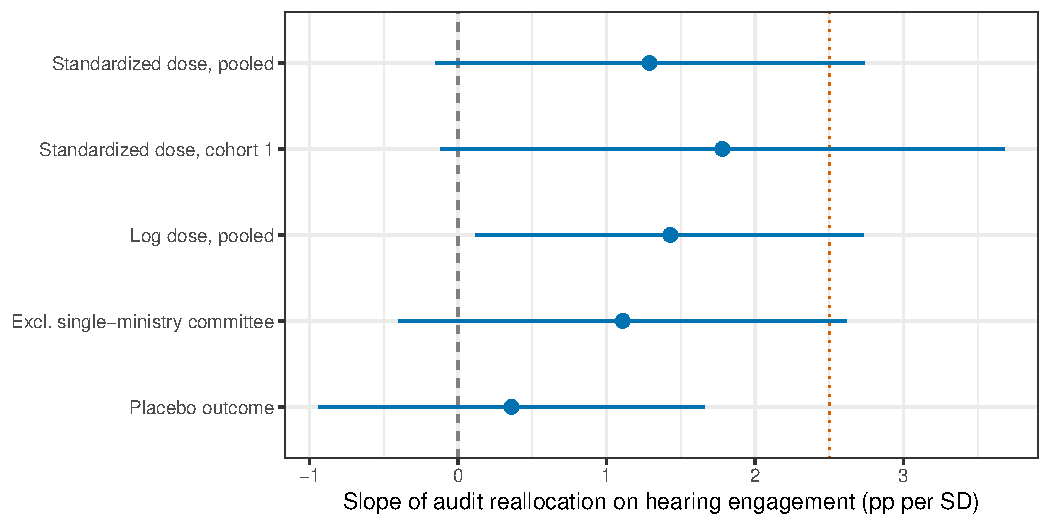
\includegraphics[width=\textwidth]{figures/2026-08-24_r27/fig_3.pdf}
\caption{Within-opposition dose slopes against the pre-set diluted-continuity bar. Points are slopes in percentage points per within-committee standard deviation of hearing engagement, and horizontal lines are 95 percent confidence intervals. The dotted line marks the 2.5-point bar.}
\label{fig:dose}
\end{figure}

The dose results land between the two theories, and the accurate classification is inconclusive. All five slopes in Table~\ref{tab:dose} are positive, and the placebo slope in column 5 is small and indistinguishable from zero, so whatever tilt exists does not appear on agencies the hearings did not touch. The top-tercile indicator, however, has a negative point estimate. No point estimate reaches the pre-set diluted-continuity bar, and two of six specifications, the log-dose variant and the raw count in cohort 1, exclude zero at the 95 percent level. With six specifications of one slope, that pattern is consistent with fragility rather than signal. Neither decision rule set before the dose estimates can fire. The survival bar of 2.5 points per standard deviation is not met by any point estimate, and the failure condition, an interval excluding that bar on a sample of at least 150 opposition pairs, cannot fire at the achievable 132. The minimum detectable effect on this sample is about 2.1 percentage points per standard deviation, so an effect of the observed magnitude cannot be resolved. The pooled 95 percent interval includes both zero and the 2.5-point bar (Table~\ref{tab:dose}, column 1, and Figure~\ref{fig:dose}), and the point estimate is about half the bar. The continuity hypothesis is weakened at this margin, not rejected, and the specialization confound discussed above gives an additional reason not to promote the residual tilt to a finding.

\subsection{Summary of Results}

Across the analyses the pattern is consistent. The carry-over prediction fails with a minimum detectable effect below the declared threshold, and the placebo estimate is also close to zero. The main estimate is equivalent to zero at the five-point threshold but not at the stricter margin. The null holds under the keyword coding, under a full change of government, and for the log-count outcome, while the named-agency outcome is positive and too imprecise to exclude the threshold. The one apparent positive finding dissolves into committee composition under a decision rule set in advance, and the intensity margin is inconclusive. Audit attention, in levels and in changes, tracks committee jurisdiction.

\section{Discussion}

Two literatures made opposite predictions for the same quantity, and the data favor the prediction of no change. Position-taking continuity, extended from \citet{mayhew1974} through the confrontation-in-oversight work of \citet{eldes2023}, predicted that a legislator who staked a public position against a nominee acquires a durable stake in that ministry's failure, raising the ministry's share of the legislator's questions at the following state audit. The Korean confirmation-hearing literature predicted instead that hearing opposition is a party-assigned role for the hearing day, discharged when the hearing ends, with audit allocation reverting to committee jurisdiction \citep{choi2008, ko2018, yoon2020}. The continuity prediction fails at the party level, with an estimate equivalent to zero at the threshold declared before estimation, and it fails again under a full change of government between audits. Within opposition questioners, the intensity margin is inconclusive. The levels of audit attention track neither hearing opposition nor its intensity but committee jurisdiction. The apparent baseline gap between opposed and supportive legislators dissolves under committee fixed effects and is matched by a larger placebo gap. Confirmation conflict and audit allocation appear to be two separate institutional routines, not a causal chain.

The adjudication is narrower than a simple victory for the party-theater account, and the narrowing deserves emphasis. The zero-change prediction of the party-theater reading held, but the reading had also seemed to gain support from the baseline levels pattern, and that support is now gone. The levels evidence turned out to discriminate for nothing except the composition of committee witness lists. The description the data license is more austere than either theory. Allocation follows jurisdiction. Party assignment may well govern who performs opposition at the hearing, as the Korean literature documents, but the performance leaves no measurable residue in the performer's subsequent allocation of oversight attention, and the party role does not even generate the standing attention premium that a strong role-based account might expect.

The results are consistent with what the political-attention literature would predict for this venue. Attention transfer into parliamentary questions is fast and short-lived, operating at the weekly-to-monthly scale \citep{walgrave2007, vliegenthart2016}, and even major focusing events produce spikes that revert within months \citep{birkland1998}. The state audit is fixed by a calendar that sets when oversight attention can be spent at all \citep{ka2025}. In cohort 1 it came five to ten months after the hearing, long enough for such attention to decay. In cohort 2 it came between five days and under five months after the hearing, which gives a partial look at shorter gaps, but with 84 pairs the cohort-2 interval is too wide to exclude the five-point threshold. A carry-over effect could therefore exist at shorter range, for instance in current-issues questioning during the weeks after appointment, and this study does not test that channel. What the study shows is that confirmation conflict does not carry into the audit at the five-point margin. The venue was fixed by the prior being tested, not chosen after the fact.

The results also refine, rather than contradict, the confrontation findings that motivated the continuity hypothesis. \citet{eldes2023} document that partisanship shapes the style of oversight questioning, with opposition-aligned members confronting witnesses at higher rates. Nothing here disputes that. The government-change cohort is instructive on exactly this point. When the opposed legislators' party moved from governing to opposition between the two audits, a shift that should transform confrontation incentives, their allocation of questions across ministries still did not move. Partisan alignment appears to govern how legislators question, while jurisdiction governs whom they question. The appointment fight changes neither. The finding similarly complements \citet{senninger2017}. Opposition scrutiny follows the strategic opportunities of the moment, and a months-old hearing position does not seem to constitute one.

Several limitations bound these conclusions. The outcome is allocation, not content. Legislators who opposed a nominee might question the confirmed ministry no more often but more aggressively, and a tone-based or confrontation-coded outcome could detect a carry-over that share-based allocation misses. That channel remains untested here. The intensity margin is unresolved. The dose slope is positive in the main specifications and small on placebo agencies, but the achievable opposition sample cannot distinguish an effect of the observed size from zero or from the pre-set bar, and the specialization confound means that even a resolved positive slope would not identify hearing-generated attention. Treatment is observational, and the primary coding is party-based. Opposition follows party, and the party-based indicator captures the assigned role rather than an individually expressed position. Each pair is observed in one audit before and one after the hearing, so pre-hearing trends cannot be examined, and the placebo share uses the same denominator as the main share, so it is not an independent check on parallel trends. The changes specification, committee fixed effects, the placebo outcome and balanced retention address some threats, but no design element delivers the counterfactual of a randomly assigned hearing antagonist. Some cells are thin. The cohort-2 supportive side contributes 32 pairs, and single-ministry committees are unusable for share outcomes, a design lesson this study learned by initially mistaking one such committee's composition for behavior. The setting, finally, is one country with a distinctive oversight calendar. The tight coupling of hearings and audits to the same standing committees is what makes the test possible, but it also fixes the interval between conflict and the next audit, and systems with continuous questioning channels might show short-range dynamics that this design cannot observe.

Finally, the trajectory of the project is part of the evidence. Two findings were overturned by decision rules set in advance. The original carry-over prior fell to its falsifier, and the baseline levels gap, at one stage the project's candidate positive finding, fell to the fixed-effects rule that had been attached to it. Both retreats were logged when they occurred. Those rules did not catch every problem. An audit after Version 1 found a coding error in cohort 2, claims about the placebo and the equivalence margins that the analysis record did not support, and secondary estimates that did not reproduce. The correction notice at the top of this version lists each change.

\section{Conclusion}

This article asked whether the conflict legislators stage over ministerial appointments carries into their subsequent oversight of the ministries those appointments fill. To test a position-taking continuity extension of the oversight literature against the party-theater reading of Korean confirmation hearings, I built hearing rosters by rule for three nominee cohorts, coded opposition from party, followed 278 legislator-ministry pairs of the first two cohorts into the audits before and after each hearing, and estimated a difference-in-differences model of audit question allocation against a threshold set before estimation. The answer is a null. The estimate is equivalent to zero at the five-point threshold, the placebo estimate is also close to zero, the result is stable across a change of government, a baseline levels gap dissolves under committee fixed effects, and the intensity margin is inconclusive. One alternative outcome, the named-agency share, is positive and too imprecise to exclude the threshold. Audit attention follows committee jurisdiction, and the appointment fight leaves no trace on it that this design can detect.

Three implications follow. Theoretically, the finding sets a scope condition on position-taking continuity. Whatever stakes a confirmation fight creates do not show up in the next audit at the five-point margin, which is consistent with the fast decay the attention literature documents, most clearly for cohort 1, whose audits came five to ten months after the hearings. For the study of the Korean National Assembly, the finding puts a measured test in place of an untested linkage between two prominent oversight institutions. For the design of confirmation hearings, the evidence gives no support to the expectation that hearing conflict improves later audit scrutiny, at least at the five-point margin, while the intensity margin remains unresolved. Confirmation hearings may serve screening, accountability, or position-taking functions on their own terms, and improving later audit scrutiny does not appear to be among them.

Future research should pursue the two channels this design could not reach. The first is short-range carry-over, in current-issues questioning during the weeks immediately after appointment, where the attention literature predicts any effect would concentrate. The second is tone, that is, whether opposed legislators question the confirmed ministry differently even if not more often. Comparative extension to systems with continuous questioning channels would test whether the null reported here is a property of appointment conflict generally or of calendars that separate conflict from oversight opportunity by months. Each extension would benefit from thresholds declared before estimation and from decision rules that are allowed to fire against the researcher.

\bigskip
\noindent\textit{This working paper was generated by AI research agents as an
experimental output. It has not been peer-reviewed or fact-checked.
Do not cite or use in any academic, policy, or professional context.}

\bibliographystyle{apsr}
\bibliography{references_r27}


\end{document}
